\section{Metodología y resultados}

En la presente experiencia se trabajó con el tablero de la Figura \ref{fig:tablero}, el cual se utilizó para energizar los elementos utilizados en el laboratorio.

\begin{figure}[H]
    \centering
    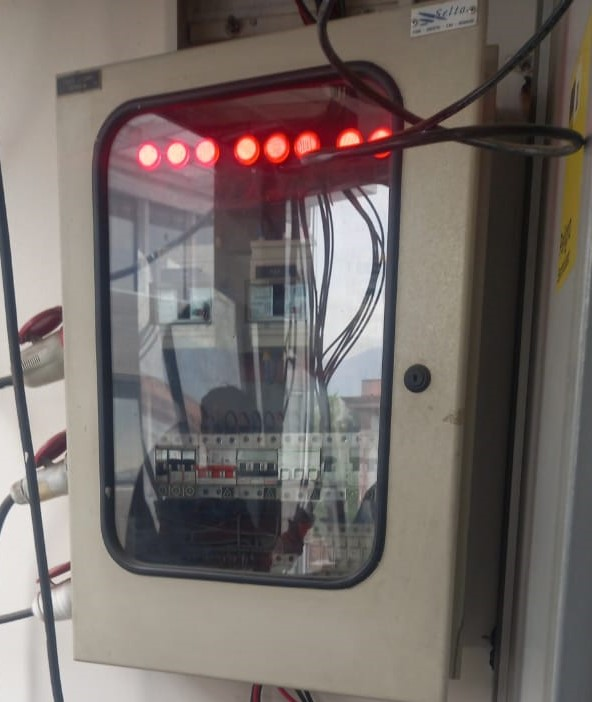
\includegraphics[width=0.4\linewidth]{img/tablero.jpg}
    \caption{Tablero eléctrico que se utilizó en la experiencia.}
    \label{fig:tablero}
\end{figure}\\

Los elementos utilizados en las actividades realizadas fueron un aerogenerador de corriente continua, un arreglo de panales solares, una microrred, un túnel de viento y un banco de ampolletas, los cuales se describirán más adelante en profundidad. Para las mediciones en corriente continua se utilizó un multímetro y una pinza amperimétrica, y para mediciones en corriente alterna se utilizó. A continuación se detallarán las actividades que se realizaron en la experiencia con sus respectivos resultados.

\subsection{Curvas Características Generación Eólica}

Con el objetivo de obtener la curva característica de potencia y viento del modelo Air X de la empresa Southwest Windpower, sé realizaron distintas mediciones de voltaje, corriente y potencia a este aerogenerador. Para esto se activó el túnel de viento que se muestra en la Figura \ref{fig:tunel} utilizando el tablero ya mencionado.

\begin{figure}[H]
    \centering
    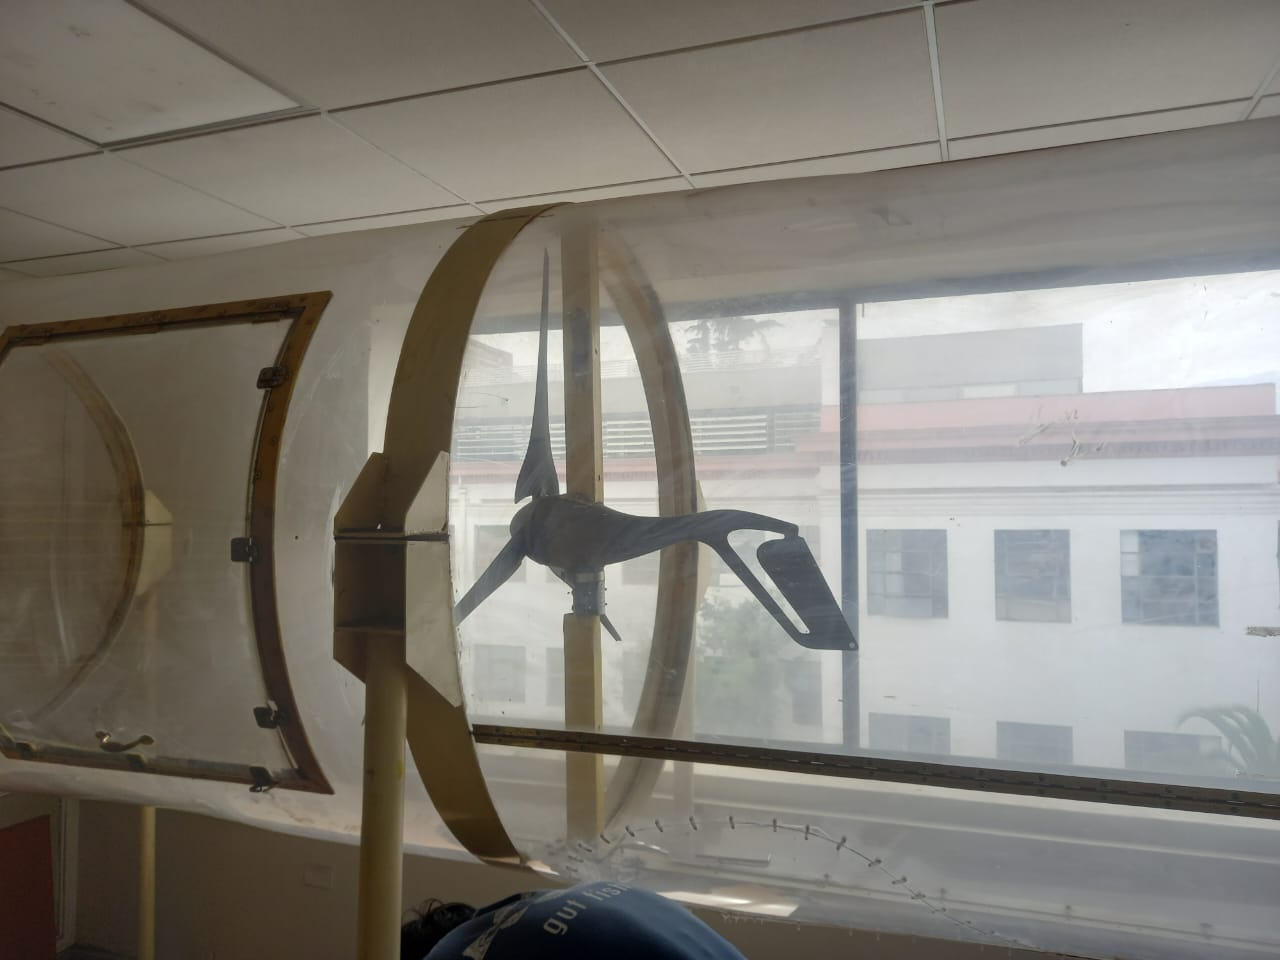
\includegraphics[width=0.5\linewidth]{img/tunel.jpg}
    \caption{Túnel de viento utilizado para controlar la velocidad de viento del aerogenerador.}
    \label{fig:tunel}
\end{figure}\\

Para las mediciones se utilizó 5 velocidades diferentes de viento usando el control de la Figura \ref{fig:control}, el cual se le fue aumentando la frecuencia en [Hz] para cambiar la velocidad de viento dentro del túnel de viento. Para cada velocidad se midió el voltaje y corriente para diferentes cargas utilizado el banco de ampolletas que se muestra en la Figura \ref{fig:ampolletas}.

\begin{figure}[H]
    \centering
    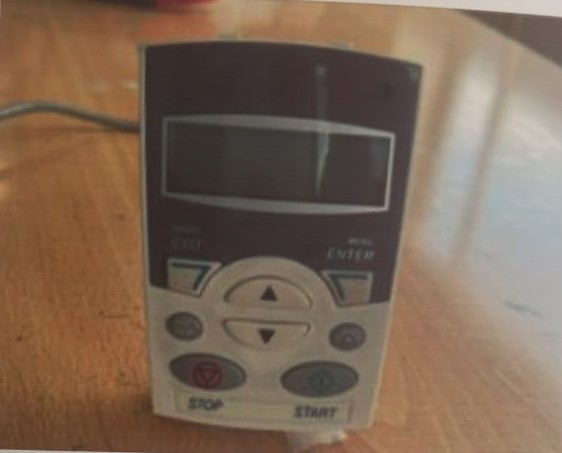
\includegraphics[width=0.5\linewidth]{img/control.jpg}
    \caption{Variador de frecuencia.}
    \label{fig:control}
\end{figure}\\

\begin{figure}[H]
    \centering
    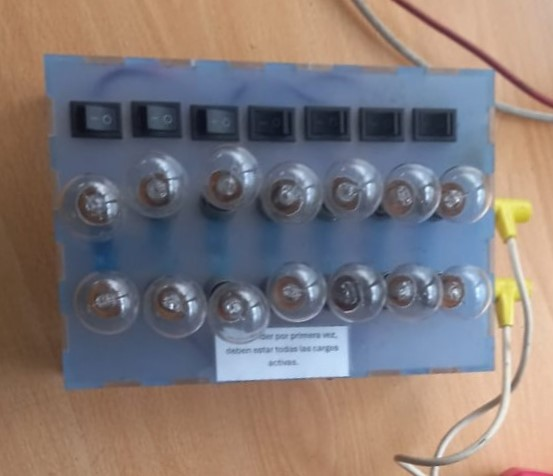
\includegraphics[width=0.5\linewidth]{img/ampolletas.jpg}
    \caption{Banco de ampolletas utilizado.}
    \label{fig:ampolletas}
\end{figure}\\

Utilizando un multímetro para medir voltaje y una pinza amperimétrica para medir la corriente, se obtuvieron los siguientes resultados para distintas velocidades expuestos en las Tablas \ref{Table 1}, \ref{Table 2}, \ref{Table 3}, \ref{Table 4} y \ref{Table 5}.

\begin{table}[H]
\centering
\caption{Mediciones experimentales a velocidad 3.4 [m/s] (16 [Hz]).}
\begin{tabular}{|l|l|l|l|}
\hline
Cargas & Voltaje [V] & Corriente [A] & Potencia [W] \\ \hline
Vacío   & 24.5 & 0    & 0       \\
Carga 1 & 14   & 1.31 & 18.34  \\
Carga 2 & 0    & 0    & 0      \\
Carga 3 & 0    & 0    & 0      \\
Carga 4 & 0    & 0    & 0      \\
Carga 5 & 0    & 0    & 0      \\
Carga 6 & 0    & 0    & 0      \\
Carga 7 & 0    & 0    & 0      \\ \hline
\end{tabular}
\label{Table 5}
\end{table}

\begin{table}[H]
\centering
\caption{Mediciones experimentales a velocidad 4.3 [m/s] (20 [Hz]).}
\begin{tabular}{|l|l|l|l|}
\hline
Cargas & Voltaje [V] & Corriente [A] & Potencia [W] \\ \hline
Vacío  & 32.2 & 0    & 0      \\
Carga 1 & 21.8 & 1.74 & 37.932 \\
Carga 2 & 0    & 0    & 0      \\
Carga 3 & 0    & 0    & 0      \\
Carga 4 & 0    & 0    & 0      \\
Carga 5 & 0    & 0    & 0      \\
Carga 6 & 0    & 0    & 0      \\
Carga 7 & 0    & 0    & 0      \\ \hline
\end{tabular}
\label{Table 1}
\end{table}

\begin{table}[H]
\centering
\caption{Mediciones experimentales a velocidad 5.9 [m/s] (25 [Hz]).}
\begin{tabular}{|l|l|l|l|}
\hline
Cargas & Voltaje [V] & Corriente [A] & Potencia [W] \\ \hline
Vacío   & 31.6 & 0    & 0      \\
Carga 1 & 31.2 & 1.94 & 60.528 \\
Carga 2 & 23.9 & 3.27 & 78.153 \\
Carga 3 & 0    & 0    & 0      \\
Carga 4 & 0    & 0    & 0      \\
Carga 5 & 0    & 0    & 0      \\
Carga 6 & 0    & 0    & 0      \\
Carga 7 & 0    & 0    & 0      \\ \hline
\end{tabular}
\label{Table 2}
\end{table}

\begin{table}[H]
\centering
\caption{Mediciones experimentales a velocidad 6.5 [m/s] (16 [Hz]).}
\begin{tabular}{|l|l|l|l|}
\hline
Cargas & Voltaje [V] & Corriente [A] & Potencia [W] \\ \hline
Vacío  & 30.5 & 0    & 0       \\
Carga 1 & 28   & 1.03 & 28.84   \\
Carga 2 & 30.5 & 3.7  & 112.85  \\
Carga 3 & 26.3 & 5.16 & 135.708 \\
Carga 4 & 18.2 & 5.6  & 101.92  \\
Carga 5 & 0    & 0    & 0       \\
Carga 6 & 0    & 0    & 0       \\
Carga 7 & 0    & 0    & 0       \\ \hline
\end{tabular}
\label{Table 3}
\end{table}

\begin{table}[H]
\centering
\caption{Mediciones experimentales a velocidad 7.0 [m/s] (35 [Hz]).}
\begin{tabular}{|l|l|l|l|}
\hline
Cargas & Voltaje [V] & Corriente [A] & Potencia [W] \\ \hline
Vacío  & 29.9 & 0    & 0       \\
Carga 1 & 26   & 1.7  & 44.2    \\
Carga 2 & 27.7 & 3.53 & 97.781  \\
Carga 3 & 30.3 & 5.6  & 169.68  \\
Carga 4 & 28.5 & 7.23 & 206.055 \\
Carga 5 & 22.4 & 7.8  & 174.72  \\
Carga 6 & 0    & 0    & 0       \\
Carga 7 & 0    & 0    & 0       \\ \hline
\end{tabular}
\label{Table 4}
\end{table}

De estas tablas se obtiene las curvas de V-I que la Figura  \ref{V-I aerogenerador}, donde el punto rojo indica el punto de máxima potencia de la curva.

\begin{images}{Curvas V-I del aerogenerador para distintas velocidades de viento. El punto rojo indica el punto de máxima potencia.}
	\addimage{img/Curva V-I (vel. viento 3.4 [m/s]).png}{width=6cm}{Curva V-I para una velocidad de viento de 3.4 [m/s].}
    \addimage{img/Curva V-I (vel. viento 4.3 [m/s]).png}{width=6cm}{Curva V-I para una velocidad de viento de 4.3 [m/s].}
	\imagesnewline
	\addimage{img/Curva V-I (vel. viento 5.9 [m/s]).png}{width=6cm}{Curva V-I para una velocidad de viento de 5.9 [m/s].}
    \addimage{img/Curva V-I (vel. viento 6.5 [m/s]).png}{width=6cm}{Curva V-I para una velocidad de viento de 6.5 [m/s].}
    \imagesnewline
	\addimage{img/Curva V-I (vel. viento 7 [m/s]).png}{width=6cm}{Curva V-I para una velocidad de viento de 7 [m/s].}
    \label{V-I aerogenerador}
\end{images}

Utilizando los puntos de máxima potencia para cada velocidad se creo el gráfico de potencia versus velocidad de viento de la Figura \ref{fig:Curva P-Vel}.

\begin{figure}[H]
    \centering
    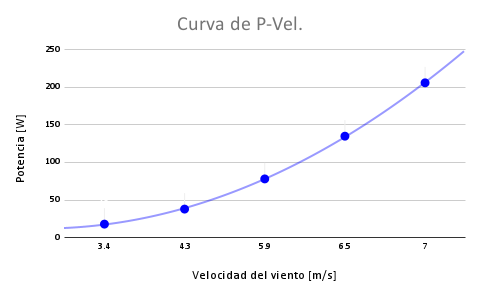
\includegraphics[width=0.5\linewidth]{img/Curva de P-Vel.png}
    \caption{Curva de potencia generada en función de la velocidad, obtenida de forma experimental.}
    \label{fig:Curva P-Vel}
\end{figure}\\

\subsection{Máxima Transferencia de Potencia Generación Solar (Operación aislada)}

Para esta actividad se activó la conexión de los paneles de la Figura \ref{fig:PV} con la sala del laboratorio, en específico con la conexión de la Figura \ref{fig:Bornes}.

\begin{figure}[H]
    \centering
    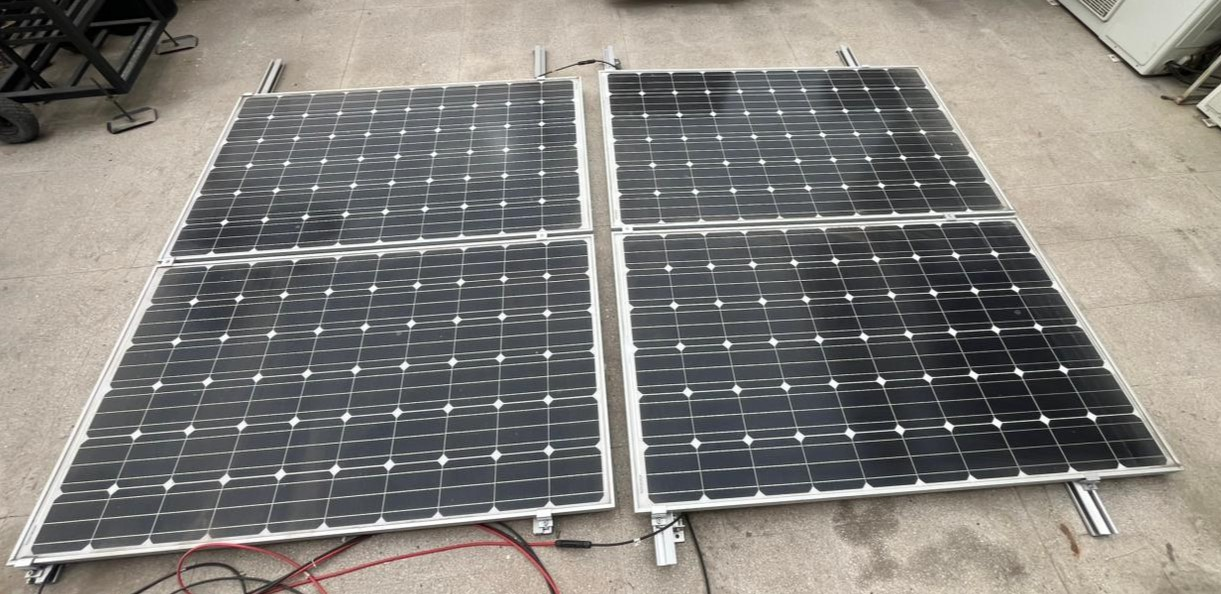
\includegraphics[width=0.5\linewidth]{img/PV.jpg}
    \caption{Paneles fotovoltaicos usados.}
    \label{fig:PV}
\end{figure}\\

\begin{figure}[H]
    \centering
    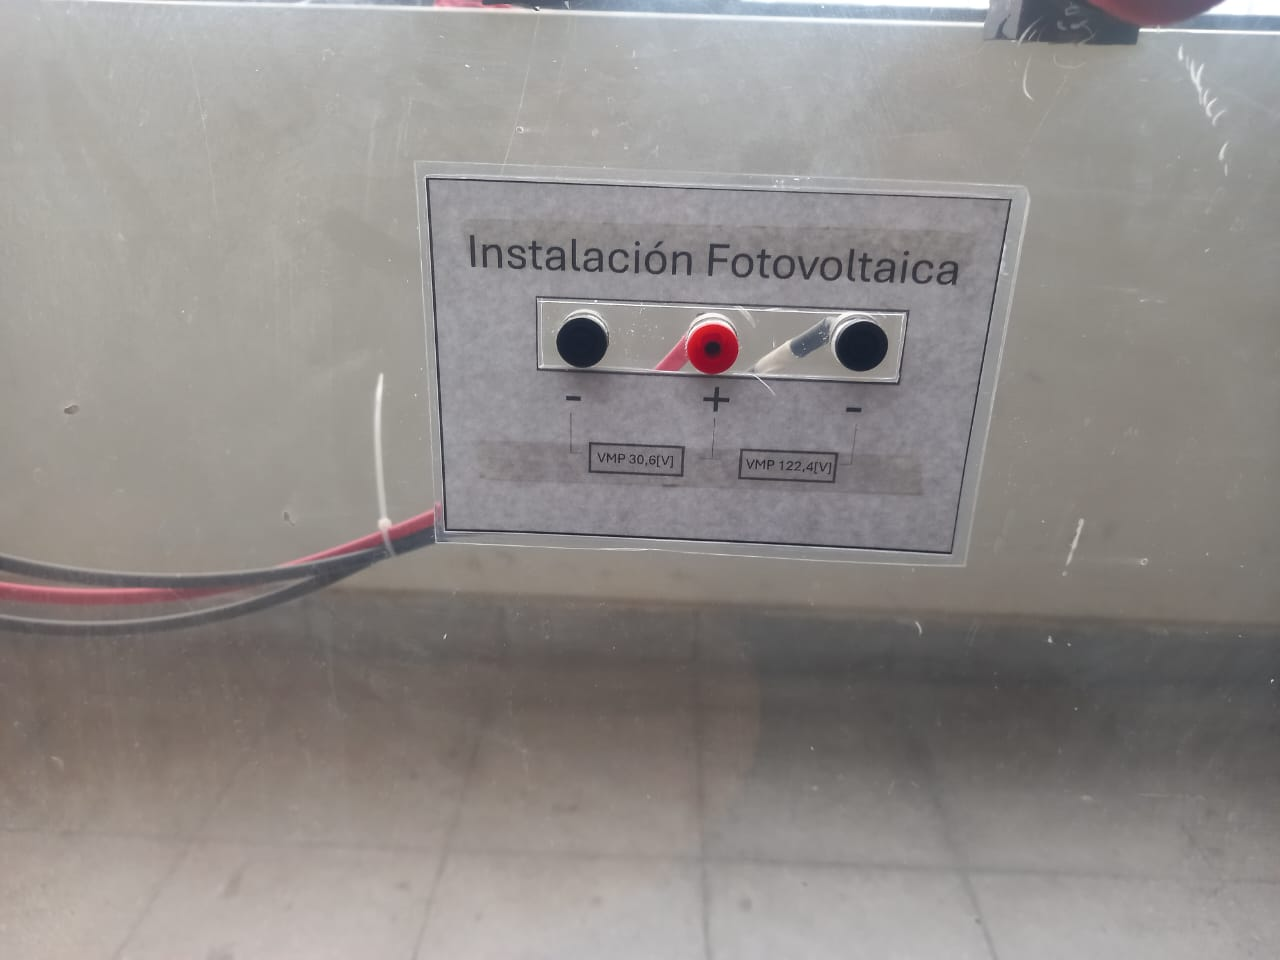
\includegraphics[width=0.5\linewidth]{img/bornes_PV.jpg}
    \caption{Bornes de los paneles PV en el laboratorio.}
    \label{fig:Bornes}
\end{figure}\\

El objetivo fue obtener la curva V-I de los paneles PV, por lo que se realizaron varias mediciones de voltaje y corriente para distintas cargas conectadas al panel PV. Para esto se utilizó nuevamente el banco de ampolleta de la Figura \ref{fig:ampolletas} conectado a los bornes para la configuración de 30.6 [V]. De esto se obtuvieron los siguientes resultados de la Tabla \ref{tabla:V-I, sin tapar}.

\begin{table}[H]
\centering
\caption{Datos del panel en operación aislada}
\begin{tabular}{|c|c|c|c|c|}
\hline
& Voltaje [V] & Corriente [A] & Potencia [W] & Hora \\ \hline
Vacío    & 35.1 & 0     & 0.00  & 10:36 \\ \hline
Carga 1  & 15.1 & 1.26  & 19.03 & 10:33 \\ \hline
Carga 2  & 4.2  & 1.31  & 5.50  & 10:34 \\ \hline
Carga 3  & 2.1  & 1.31  & 2.75  & 10:34 \\ \hline
Carga 4  & 1.3  & 1.31  & 1.70  & 10:35 \\ \hline
Carga 5  & 1.3  & 1.306 & 1.70  & 10:35 \\ \hline
Carga 6  & 1.2  & 1.00  & 1.57  & 10:35 \\ \hline
Carga 7  & 1.1  & 1.00  & 1.44  & 10:36 \\ \hline
Corto    & 0    & 1.00  & 0.00  & 10:37 \\ \hline
\end{tabular}
\label{tabla:V-I, sin tapar}
\end{table}

Con estos datos se creo la cura de V-I de la Figura \ref{fig:curva v-i sin tapar}.

\begin{figure}[H]
    \centering
    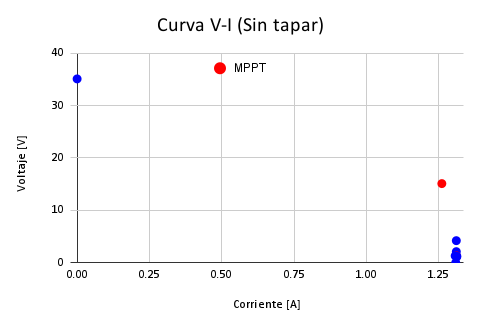
\includegraphics[width=0.5\linewidth]{img/Curva V-I (Sin tapar).png}
    \caption{Curva V-I del panel PV.}
    \label{fig:curva v-i sin tapar}
\end{figure}\\

\subsection{Máxima Transferencia de Potencia Generación Solar (Operación en red)}

En esta actividad se activa la microrred mediante el tablero y se hace uso del inversor de las Figuras \ref{fig:red} y \ref{fig:inversor}.

\begin{figure}[H]
    \centering
    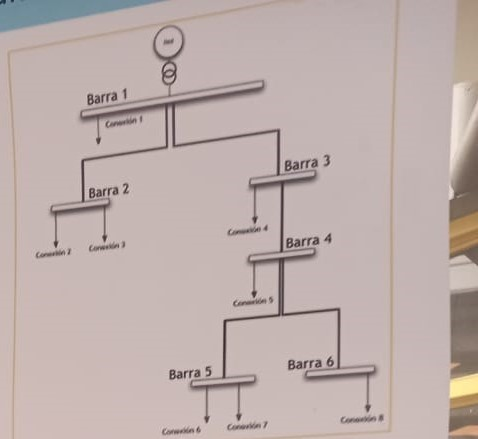
\includegraphics[width=0.4\linewidth]{img/red.jpg}
    \caption{Diagrama de la microrred.}
    \label{fig:red}
\end{figure}\\

\begin{figure}[H]
    \centering
    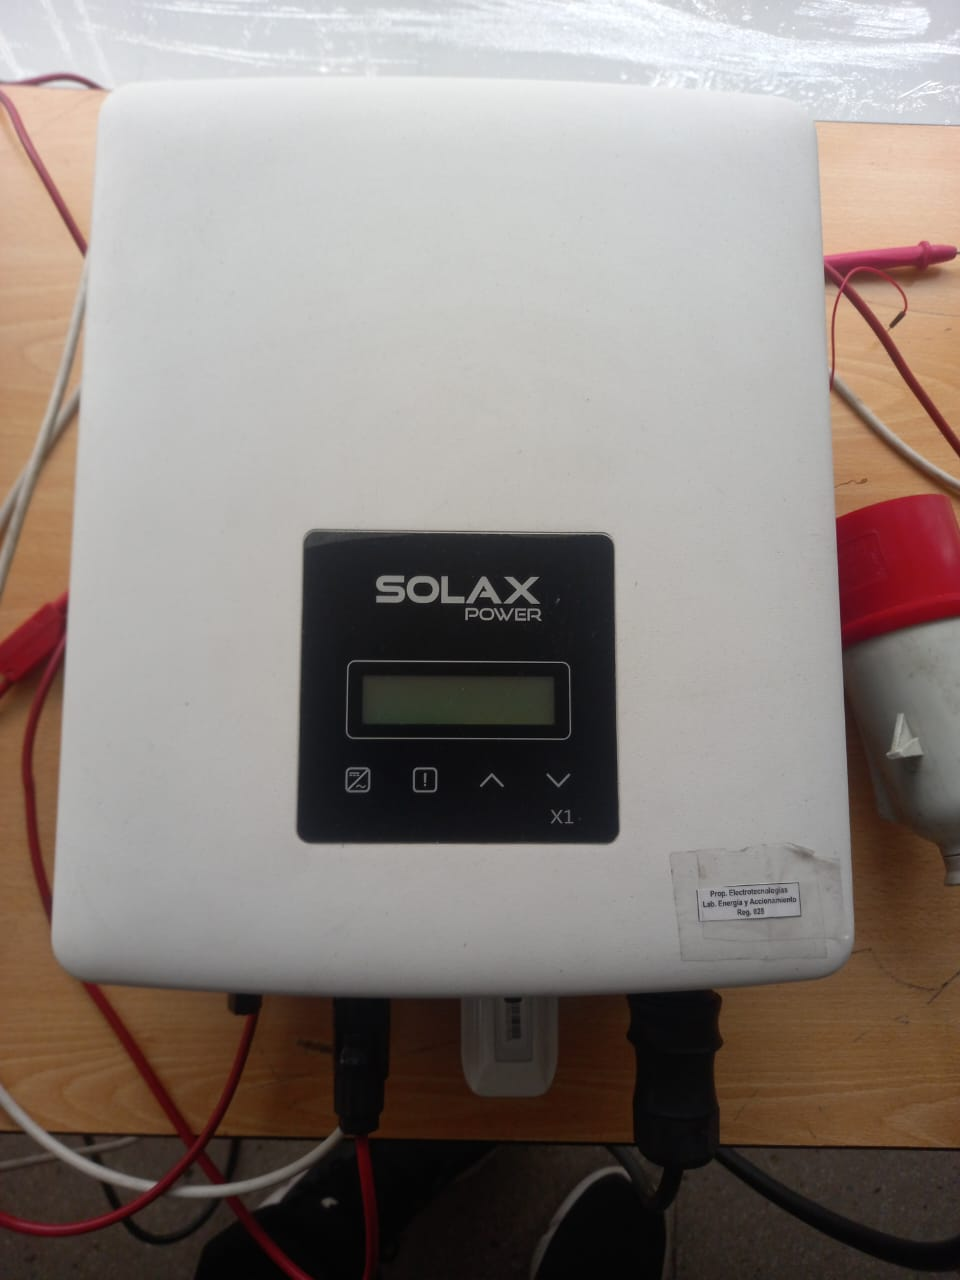
\includegraphics[width=0.4\linewidth]{img/inversor.jpg}
    \caption{Inversor utilizado.}
    \label{fig:inversor}
\end{figure}\\

Se conecta la entrada del inversor a la conexión de 122.4 [V] de la Figura \ref{fig:Bornes} y su salida a la barra 5 de la Figura \ref{fig:SEP} (se utiliza esta barra para poder medir armónicos).

\begin{figure}[H]
    \centering
    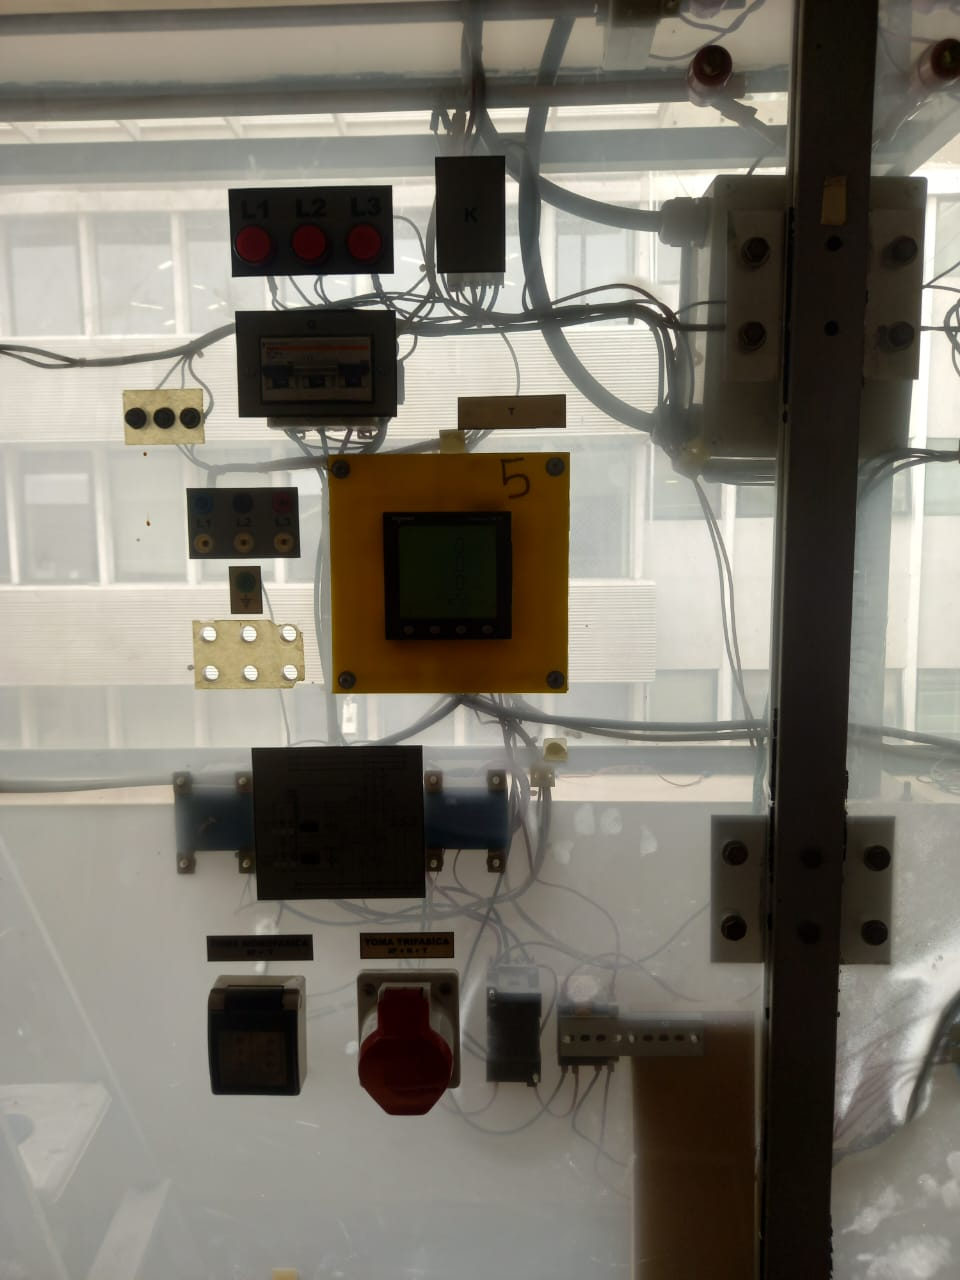
\includegraphics[width=0.4\linewidth]{img/SEP.jpg}
    \caption{Barra 5 de la microrred utilizada.}
    \label{fig:SEP}
\end{figure}\\

Se activa la barra 5 mediante el programa OPC Client y se miden los datos de la Tabla \ref{tabla:AC} mediante el programa Enervista.

\begin{table}[H]
\centering
\caption{Datos del panel en operación en red.}
\begin{tabular}{|l|c|}
\hline
\textbf{Parámetro} & \textbf{Valor} \\ \hline
Voltaje DC [V]     & 1255     \\ \hline
Corriente DC [A]   & 2.95     \\ \hline
Voltaje AC [V]     & 406      \\ \hline
Frecuencia [Hz]    & 50.028   \\ \hline
Potencia [W]       & 294      \\ \hline
THD                & 18.6     \\ \hline
Factor de potencia & 0.999 ind\\ \hline
Hora de comienzo   & 11:05    \\ \hline
Hora de término    & 11:08   \\ \hline
\end{tabular}
\label{tabla:AC}
\end{table}


\subsection{Efecto Sombra}

En esta actividad se repiten las dos anteriores, pero con un panel tapado parcialmente, como se observa en la Figura \ref{fig:Curva V-I tapado}.

\begin{figure}[H]
    \centering
    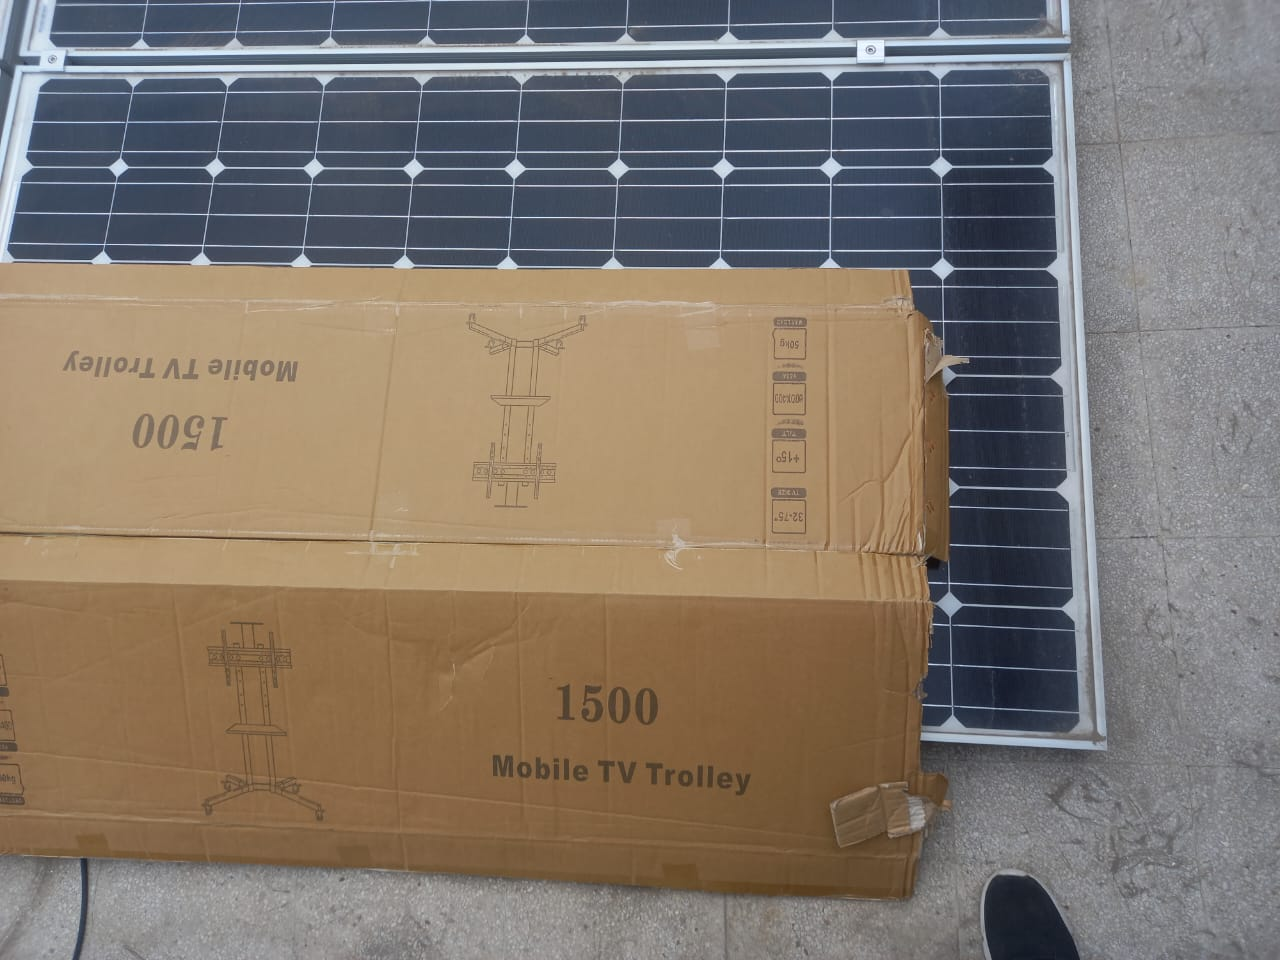
\includegraphics[width=0.5\linewidth]{img/panel tapado.jpg}
    \caption{Panel PV parcialmente cubierto.}
    \label{fig:Curva V-I tapado}
\end{figure}\\

En operación aislada se obtuvo la siguiente Tabla \ref{tabla:dc tapado} junto a la curva de la Figura \ref{fig:Curva V-I tapado}.

\begin{table}[H]
\centering
\caption{Datos del panel en operación aislada (Panel tapado).}
\begin{tabular}{|l|c|c|c|c|}
\hline
 & Voltaje [V] & Corriente [A] & Potencia [W] & Hora \\ \hline
Vacío    & 30.1 & 0.00 & 0.00  & 10:42 \\ \hline
Carga 1  & 9.7  & 1.06 & 10.30 & 10:45 \\ \hline
Carga 2  & 5.9  & 1.59 & 9.39  & 10:45 \\ \hline
Carga 3  & 2.8  & 1.60 & 4.47  & 10:46 \\ \hline
Carga 4  & 1.8  & 1.61 & 2.89  & 10:46 \\ \hline
Carga 5  & 1.6  & 1.63 & 2.61  & 10:46 \\ \hline
Carga 6  & 1.5  & 1.64 & 2.46  & 10:46 \\ \hline
Carga 7  & 1.5  & 1.65 & 2.47  & 10:46 \\ \hline
Corto    & 0.00 & 1.49 & 0.00  & 10:43 \\ \hline
\end{tabular}
\label{tabla:dc tapado}
\end{table}

\begin{figure}[H]
    \centering
    \includegraphics[width=0.5\linewidth]{img/Curva V-I (Panel  tapado).png}
    \caption{Curva V-I del panel PV con el panel tapado.}
    \label{fig:Curva V-I tapado}
\end{figure}\\

Para la operación en red se obtuvieron los siguientes resultados de la Tabla \ref{tabla:AC tapado}.

\begin{table}[H]
\centering
\caption{Datos del panel en operación en red (Panel tapado).}
\begin{tabular}{|l|c|}
\hline
\textbf{Parámetro} & \textbf{Valor} \\ \hline
Voltaje DC [V]     & 102.5   \\ \hline
Corriente DC [A]   & 1.59    \\ \hline
Voltaje AC [V]     & 406     \\ \hline
Frecuencia [Hz]    & 50.41   \\ \hline
Potencia [W]       & 206     \\ \hline
THD                & 18.9    \\ \hline
Factor de potencia & 0.997 ind \\ \hline
Hora de comienzo   & 10:48   \\ \hline
Hora de término    & 11:05   \\ \hline
\end{tabular}
\label{tabla:AC tapado}
\end{table}